\section{Introduction}
\label{sec:intro}

The rapid development of multimodal large language models (MLLMs)~\cite{qwen2vl,chen2024internvl,zhu2025internvl3} has created a growing demand for high-quality, unified visual representations. A key challenge in this field lies in aligning visual signals into a form that can be seamlessly interpreted by language models. Early and dominant approaches have primarily relied on continuous visual encoders~\cite{zhai2023siglip, radford2021clip, fini2025multimodal}, pre-trained through contrastive vision-language learning, or specialized encoders fine-tuned for multimodal tasks~\cite{chen2412expanding,qwen2vl,liu2024oryx}. Although this paradigm has achieved considerable success, it introduces a fundamental representational discrepancy: the continuous nature of visual features is intrinsically mismatched with the discrete token-based modeling of text. Furthermore, the computational process of extracting high-dimensional visual features places significant hardware strain during model training.

\begin{figure}[t]
\centering
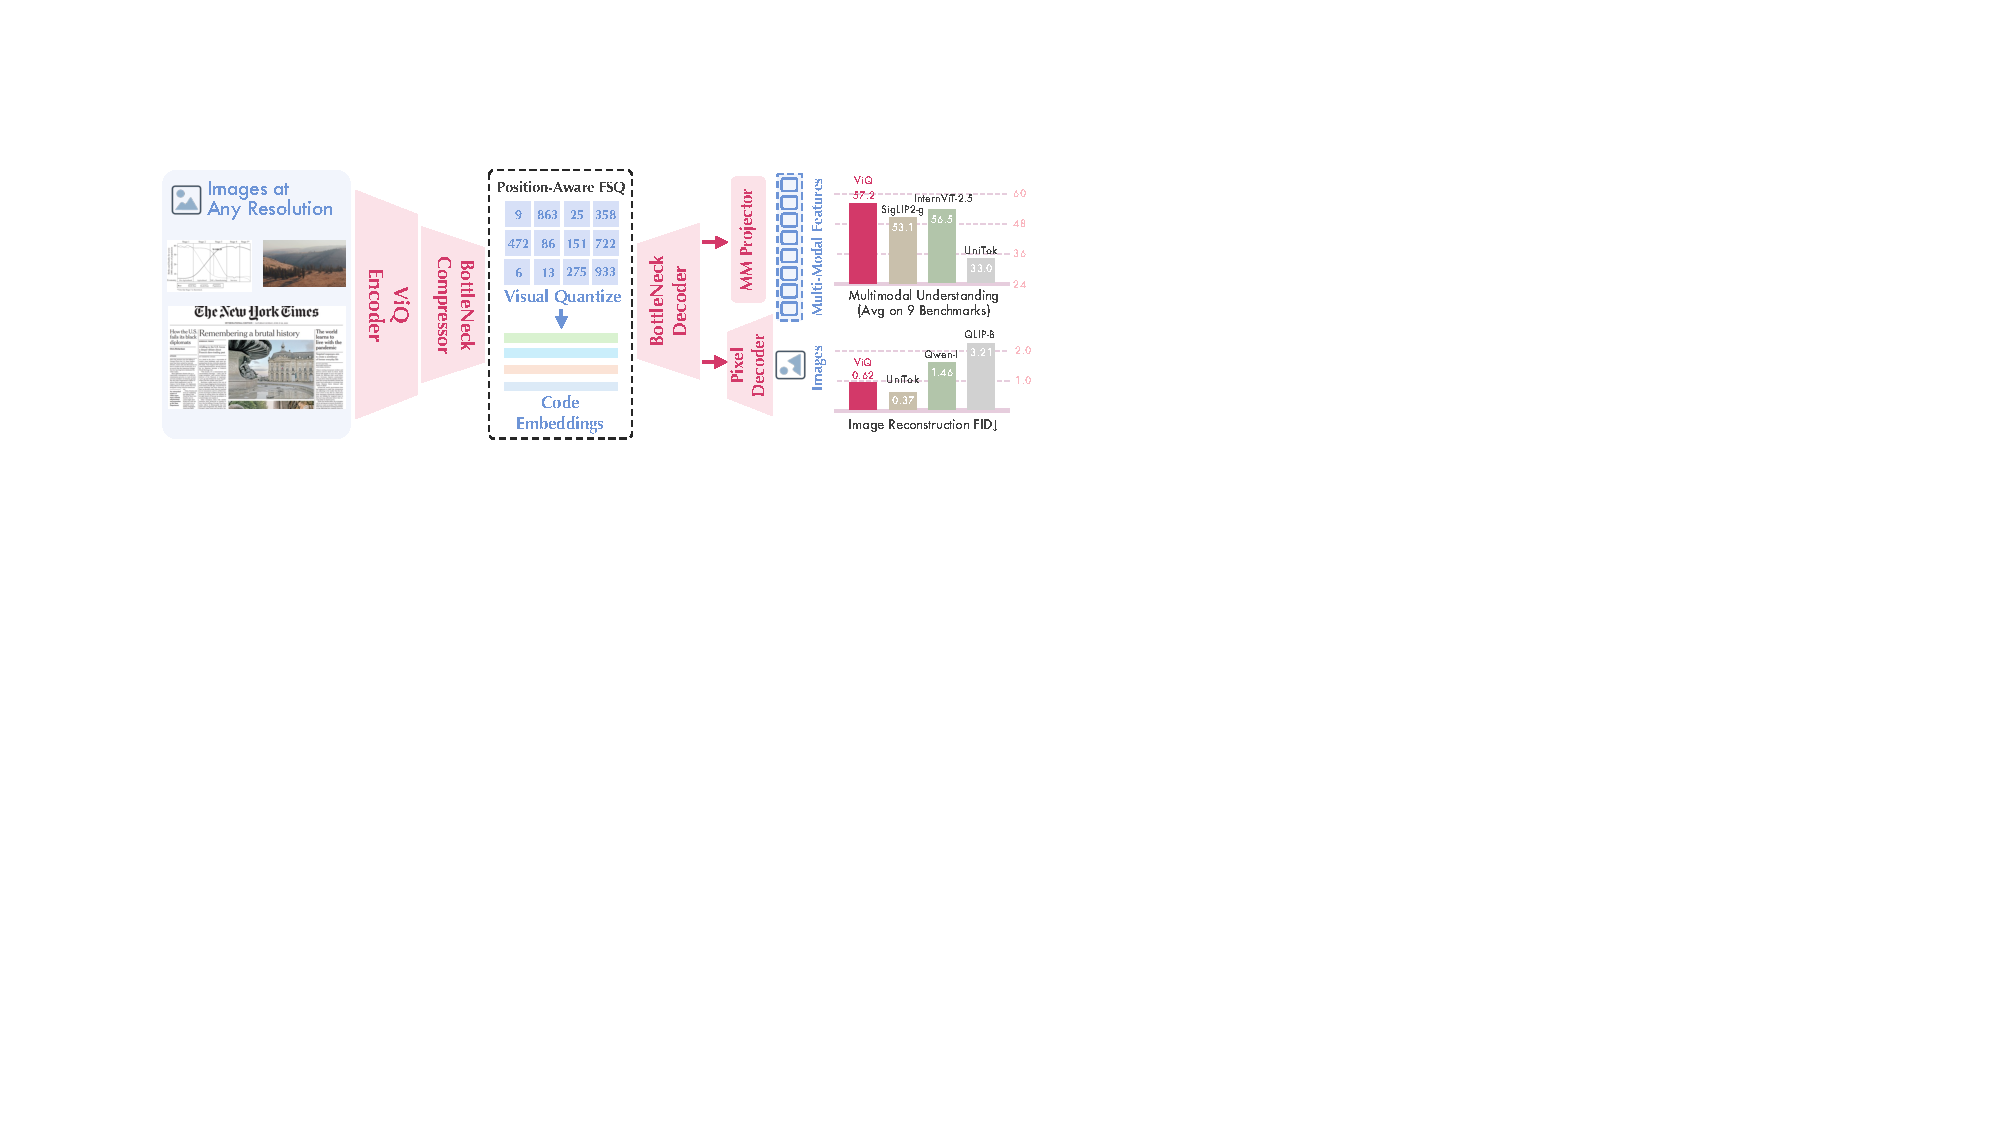
\includegraphics[width=1.0\linewidth]{figures/fig1_eccv.pdf}\vspace{-5pt}
\caption{\textbf{ViQ delivers high-quality multimodal quantized representations with both high-level semantics and low-level details.} The quantized visual codes in ViQ support high-level multimodal understanding and low-level image reconstruction, with state-of-the-art performance compared with continuous visual encoders.}
\label{fig:teaser}
\end{figure}

Inspired by the success of vector quantization~\cite{gersho2012vector,mentzerfinite,yulanguage} in visual representation learning, a growing body of research has begun exploring discrete visual representations in multimodal domains~\cite{ma2025unitok,zhao2025qlip}. These approaches typically quantize visual inputs into a finite set of discrete tokens, analogous to words in a textual vocabulary. However, a fundamental challenge remains in balancing low-level visual details with high-level semantic information. Reconstruction-focused autoencoders often fail to preserve semantic structure in their latent features, while semantically rich visual encoders tend to incur significant information loss during quantization. This creates a critical gap in multimodal representations, which require both fine-grained visual details and rich semantic content to handle complex tasks effectively. As a result, the application of quantized visual encoders has been largely limited, and they have yet to match the high fidelity and robustness of continuous encoders in demanding real-world scenarios.

To address this issue, we propose ViQ (Visual Quantized Representations), a novel approach that elevates the performance of discrete visual representations in multimodal tasks to a level comparable with widely-used continuous features, while supporting native-resolution visual inputs. Our method structures quantization learning into two phases: text-aligned pre-training and visual quantization learning. In the initial stage, the ViQ model learns semantically rich alignments through supervision from vision-language pairs. To mitigate information loss during quantization, we introduce a proximal representation learning strategy that constrains the latent visual space, followed by a quantization mechanism enhanced with position encoding and expanded visual features. This design supports quantization at arbitrary resolutions and improves the representational capacity of visual codes. Our work not only strongly enhances the efficiency of multimodal encoders in training process but also unifies visual and linguistic representations into a cohesive discrete framework.

We evaluate the ViQ model against state-of-the-art continuous multimodal visual encoders and quantized multimodal semantic encoders across a range of experiments. Under consistent fine-tuning data and training protocols, ViQ not only outperforms existing quantized models by a large margin but also achieves competitive results compared to well-established continuous encoders such as InternViT~\cite{zhu2025internvl3}, AIMv2~\cite{fini2025multimodal}, and SigLIP2~\cite{tschannen2025siglip}. On the aggregated score over nine benchmarks—spanning visual question answering, world knowledge, and document and chart recognition—ViQ attains an average of 57.2 with Qwen2.5-1.5B as the backbone LLM and 63.9 with Qwen2.5-7B, surpassing the previous state-of-the-art scores of 57.0 and 63.8, respectively, under 6B number of visual encoder parameters. The quantized representation also brings substantial efficiency gains in real-world multimodal training. Compared to conventional training strategies, using the ViQ visual encoder yields speedups of 20\% to 70\% in training recipes varying in sequence lengths. Furthermore, ViQ preserves rich low-level visual details: when fine-tuned with an image decoder, it achieves a PSNR of 22.73 and an rFID score of 0.62, ranking first among mainstream discrete visual autoencoders. This strong performance in both understanding and reconstruction tasks underscores the effectiveness and unity of our discrete representation.
